\subsection{Wizualizacja}
Wizualizacja modeli 3D stanowi wyzwanie dla użytkownika końcowego,
głównie z powodu braku spójnych platform umożliwiających realizację
całego procesu – od wgrania plików wejściowych po interakcję z modelem – w ramach jednej aplikacji.
Dostępne na rynku rozwiązania wymagają korzystania z aplikacji trzecich i pewnej wiedzy technicznej,
co prowadzi do problemów z integracją i spójnością działania.

Celem projektu było stworzenie intuicyjnego, dynamicznego i responsywnego \textbf{interfejsu} zintegrowanego z wydajnym \textbf{renderingiem} GPU.
Aplikacja umożliwia użytkownikowi końcowemu realizację pełnego procesu
wizualizacji – od tworzenia i modyfikacji modelu po jego segmentację i wyświetlanie – w jednej aplikacji.
Projekt rozwiązuje problem fragmentarycznej funkcjonalności dostępnych aplikacji, oferując spójne środowisko do obsługi modeli 3D.

\textbf{Korzyści z realizacji interfejsu}

\begin{itemize}
    \item zwiększona wydajność dzięki GPU,
    \item eliminacja konieczności korzystania z wielu narzędzi,
    \item uproszczony proces użytkowania, co zwiększa dostępność aplikacji dla mniej zaawansowanych użytkowników.
\end{itemize}

Rendering wykorzystuje plik .ply jako dane wejściowe do wczytania splatów.
Są one renderowane jako sześciany, w których wnętrzu generowane są shadery, bazujące na skalowaniu i rotacji splatów.
Takie podejście umożliwia abstrakcyjne przedstawienie splatów przy jednoczesnym zachowaniu wysokiej dokładności wizualnej.

Interfejs widoczny na ilustracji \ref{fig:ui} został zaimplementowany w \textit{QML}, \textit{PyQt}, natomiast rendering w technologiach \textit{C}, \textit{OpenGL} oraz \textit{OpenCL}, przedstawiony na zdjęciu \ref{fig:rendering}. Tymczasową wizualizację chmury wykonywaliśmy przy pomocy biblioteki \textit{VisPy}.


\begin{figure}[!ht]
    \centering
    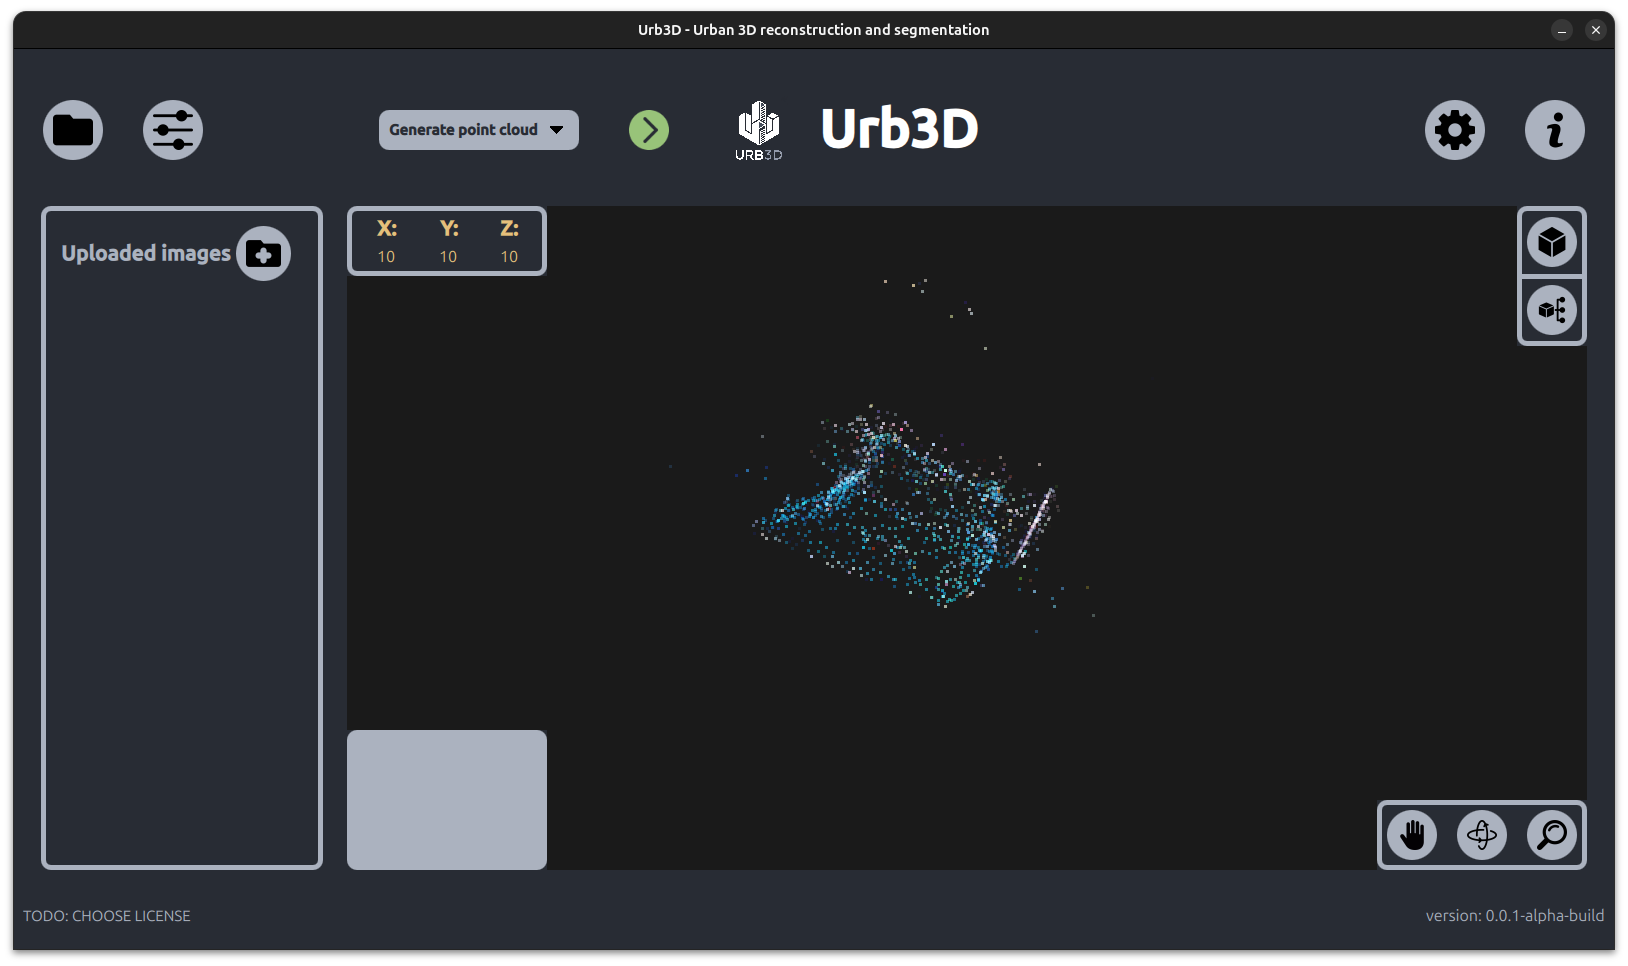
\includegraphics[width=\textwidth]{images/UI-Rendering.png}
    \caption{Zrzut ekranu przedstawiający główny widok aplikacji}
    \label{fig:ui}
\end{figure}

\begin{figure}[!ht]
    \centering
    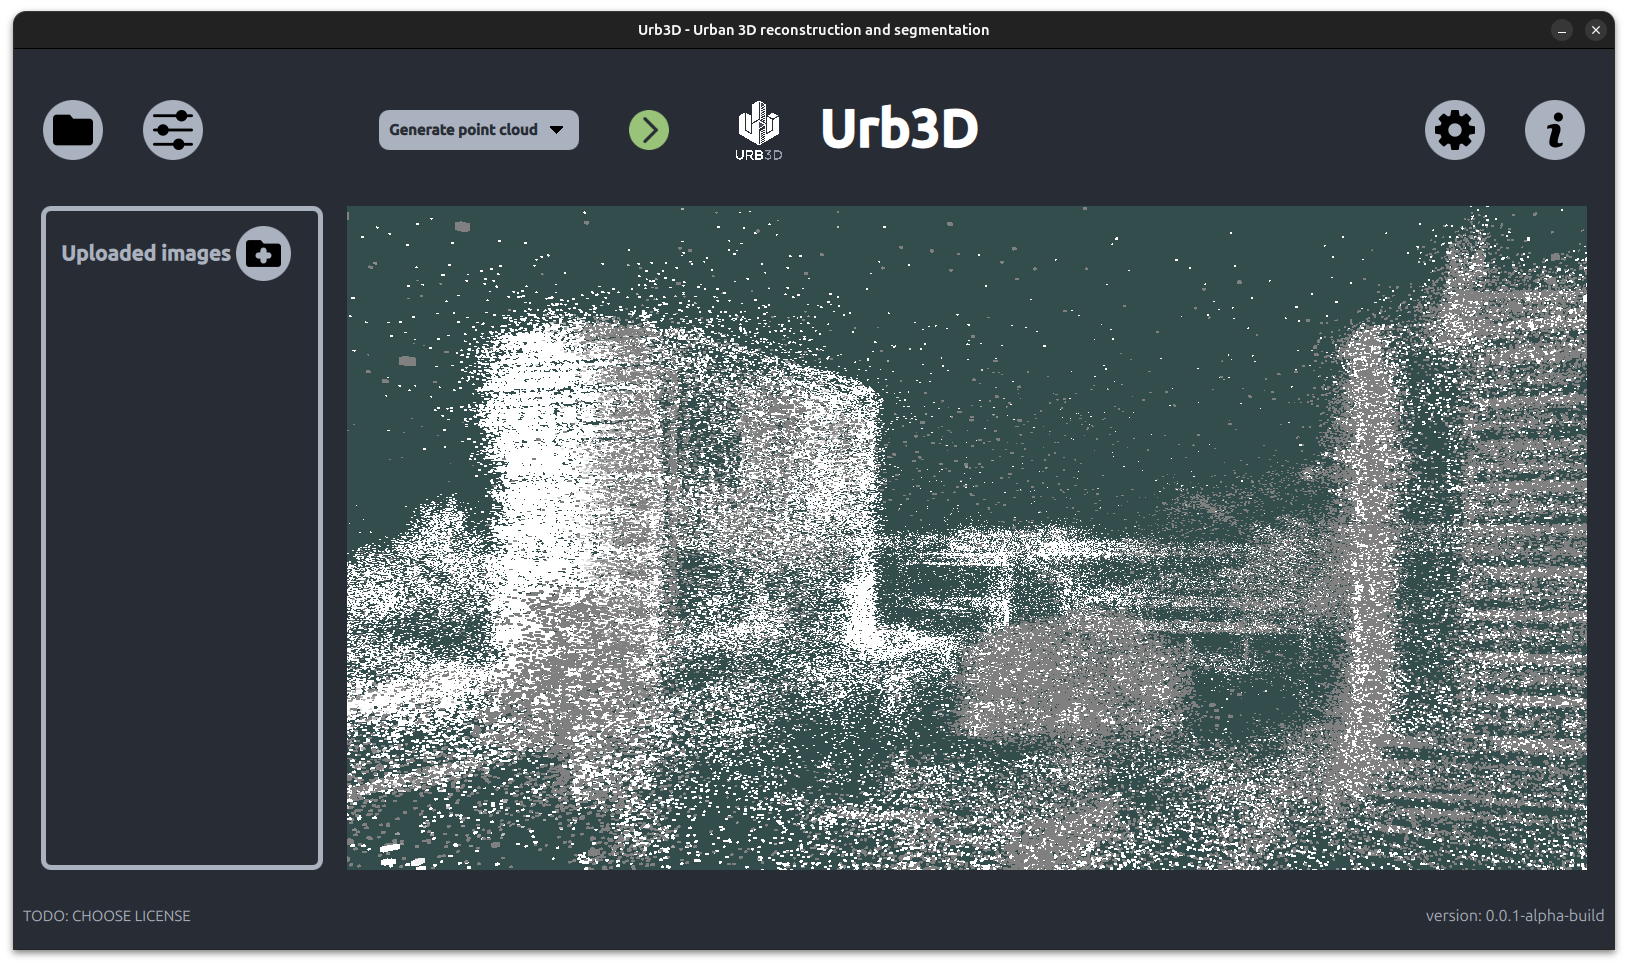
\includegraphics[width=\textwidth]{images/cloud_rendering.png}
    \caption{Zrzut ekranu przedstawiający własny renderer}
    \label{fig:rendering}
\end{figure}
